% (approx. 500-800 words)

\section{Evaluation}
\label{sec:eval}
This section will showcase results from different runs. In particular, it is worth mentioning that some default hyper-parameters were used, such as:
\begin{itemize}
    \item \textit{batch size} set to $128$ samples both for training the BiSTM and for the final polarity evaluation procedure and to $64$ 
        samples for the  binary classifier;
    \item concerning the \textit{dataset split} dimensions:
        \begin{itemize}
            \item the subjectivity dataset was split into training set ($80\%$) and test set ($20\%$). The training set has been further splitted 
            with a  randomly sampled $10\%$ for evaluation pruposes;
            \item the IMDB dataset has been splitted following the built-in format of the dataset itself ($25'000$ samples for training
            and $25'000$ samples for evaluation)
        \end{itemize}
    \item during the training procedure an \textit{early stopper} has been used to implement early stopping. To achieve it, the 
        difference between the accuracy of the previous run and the current one is investigated. If the latter is grater than $MIN\_DELTA=0.075$, 
        the training procedure is interrupted and the last model saved;
    \item the BiLSTM model has been trained for $10$ \textit{epochs} and the binary classifier just for one (for time reasons);
    \item regarding the BiLSTM model, the multiple runs have been performed using  randomly selected seeds: $[91, 11, 57, 822, 19]$;
    \item for the AdamW and Adam optimizers, the learning rates used are $0.001$ and $0.0002$ respectively. 
\end{itemize}


\subsection{Evaluation metric}
\label{subsec:metric}
Across the different models, several evaluation metrics have been used. 
\vspace{-1.0em}
\subsubsection{Baseline}
For the baseline, a simple \texttt{accuracy} metric has been used across a 10-fold cross validation procedure.
\vspace{-.5em}
\subsubsection{Custom model}
Regarding my proposed model, different evaluation metrics have been used for the different components:
\begin{itemize}
    \item for the BiLSTM model a simple cumulative accuracy metric, which is the sum of all batches' agreements over the number of samples in the training set, has been used;
    \item for the \texttt{BertForSequenceClassification} instance an ensamble of metrics has been computed, exploiting the 
    \texttt{accuracy\_score} and \texttt{precision\_recall\_fscore\_support} methods provided by the \texttt{sklearn} python module. 
    In particular, the function used to compute these metrics can be analysed in \textbf{\Cref{alg:binaryclf}}
    \item as for the BiLSTM model, in the final polarity classification step a cumulative accuracy has been used, where the agreements
    between the predictions given by the pre-fine-tuned binary classifier and the ground truth are investigated and quantified.
\end{itemize}

\vspace{-1.0em}
\begin{algorithm}[!h]
    \SetAlgoLined
    \DontPrintSemicolon
    \KwIn{pred}    
    \KwOut{accuracy, f1, precision, recall}
    \CommentSty{\color{blue}}
    precision, recall, f1, \_  $\gets$ precision\_recall\_fscore\_support(labels, preds, average='binary')\;
    acc $\gets$ accuracy\_score(labels, preds)\;

    return\{
            'accuracy': acc,\;
            \hspace{10mm}'f1': f1,\;
            \hspace{10mm}'precision': precision,\;
            \hspace{10mm}'recall': recall
        \}

\caption{Metric computation function used in Trainer interface.}
\label{alg:binaryclf}

\end{algorithm}

Of course, the overall objective is to maximise the accuracy on both subjectivity and polarity datasets by minimizing the losses used during the training procedure and 
finding the best possible set of weights. 

\subsection{Results}
\label{subsec:res}
In this particular section, the results obtained across different runs and experiments are analysed. 
\begin{figure}
    \centering
    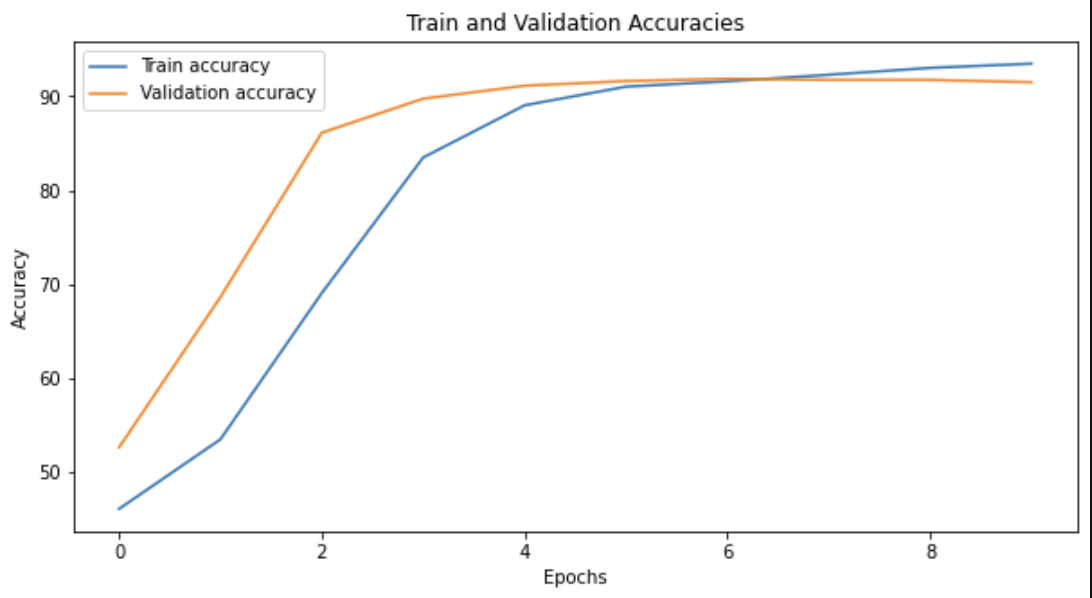
\includegraphics[scale=0.28]{Images/singlerunacc.png}
    \vspace{-1.0em}
    \caption{BiLSTM model training and evaluation accuracies on a single run.}
    \label{fig:singlerunacc}
    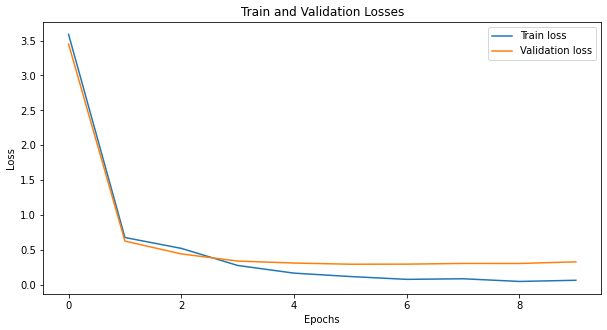
\includegraphics[scale=0.28]{Images/singlerunloss.png}
    \vspace{-1.0em}
    \caption{BiLSTM model training and evaluation losses on a single run.}
    \label{fig:singlerunloss}
    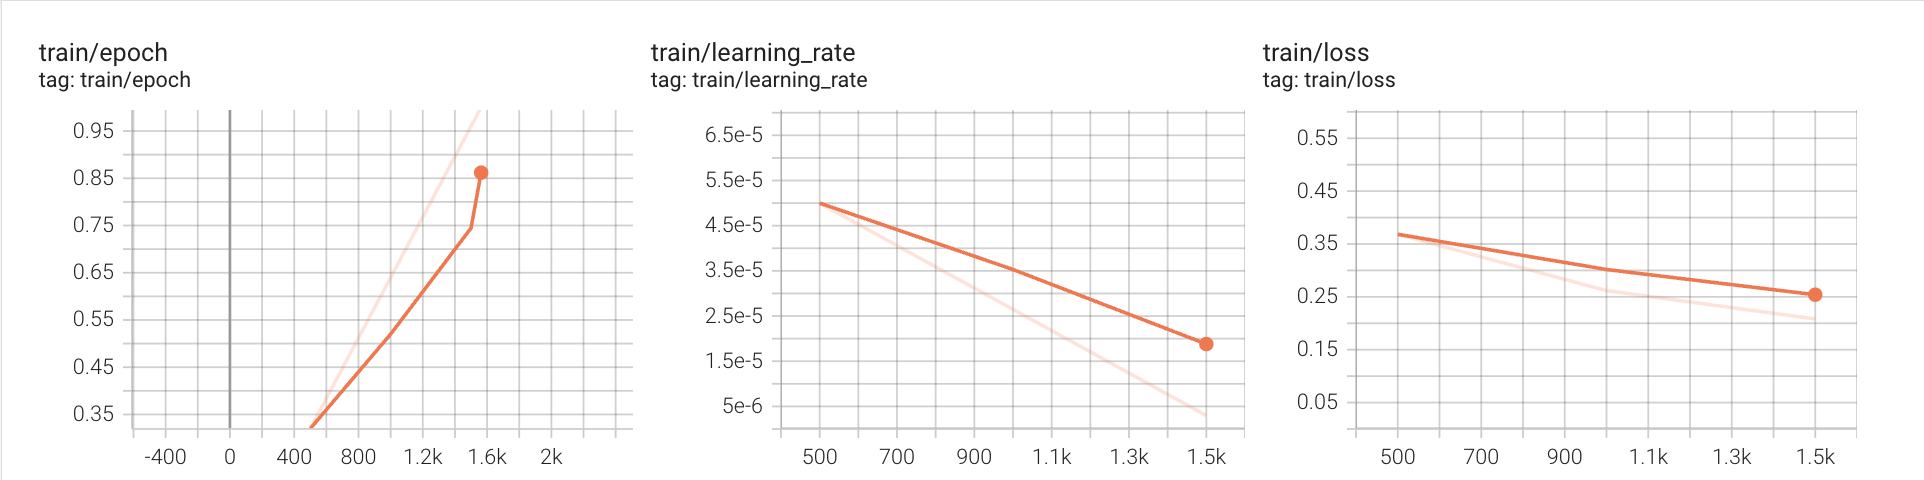
\includegraphics[width=0.5\textwidth]{Images/BinaryCLF.png}
    \vspace{-1.0em}
    \caption{Binary classifier statistics.}
    \vspace{-1.0em}
    \label{fig:singleepoch}
\end{figure}


In \textbf{\Cref{fig:singlerunacc}} and \textbf{\Cref{fig:singlerunloss}} it is possible to appreciate the training and 
evaluation accuracies and losses respectively, on a single run for the BiLSTM model (discussed in \textbf{\Cref{subsec:custom}}). \\
Since a single run is not expressive and reliable enough, I decided to perform a 5-fold cross validation addressing both the average 
accuracy as well as the variance across the different runs (for details refer to \textbf{\Cref{tab:crossval}}).\\

\begin{center}
        \vspace{-4.0em}
        \begin{table}
            \let\TPToverlap=\TPTrlap    
            \centering
            \caption{5-fold cross validation subjectivity results using BiLSTM model}
            \vspace{-1.0em}
            \begin{threeparttable}
                    \begin{tabular}{cc}
                        \toprule
                        \thead{Seeds} & \thead{Accuracy} \\
                        \hline
                        $91$ & $89.45$ \\
                        $11$ & $90.35$ \\
                        $57$ & $90.85$\\
                        $822$ & $89.45$\\
                        $19$ & $89.2$ \\
                        \hline
                        Avg. Acc. & $89.86$ \\
                        \hline
                        Acc. Var. & $0.63$ \\
                        \bottomrule
                    \end{tabular}
                \label{tab:crossval}
            \end{threeparttable}
        \end{table}
\end{center}

The main reason behind using a BiLSTM model is to try to better catch the dependencies between the words in a sentence. The results turned out to be worse than the ones
obtained with the baseline for cumulative accuracy, but better in terms of consistency and stableness. Indeed, using the same evaluation metric, the average
statistics, listed in \textbf{\Cref{tab:comparison}}, show that the baseline reaches a better average accuracy but a higher variance across the different runs, i.e. 
seems to be more unstable and inconsistent.\\

\begin{center}
        \vspace{-4.0em}
        \begin{table}
            \let\TPToverlap=\TPTrlap    
            \centering
            \caption{Comparison between the baseline and the BiLSTM model}
            \vspace{-1.0em}
            \begin{threeparttable}
                    \begin{tabular}{ccc}
                        \toprule
                        \thead{Model} & \thead{Accuracy} & \thead{Variance}\\
                        \hline
                        Baseline & $90.75\%$ & $0.00013765$ \\
                        Custom Model & $89.86\%$ & $5.534000000000004e-05$\\
                        \bottomrule
                    \end{tabular}
                    \label{tab:comparison}
            \end{threeparttable}
        \end{table}
\end{center}

Investigating the final results on the polarity dataset, we can notice that the proposed model reaches a better accuracy than the baseline, as shown in 
\textbf{\Cref{tab:finalres}}.\\ It is worth mentioning that the "x" on the \texttt{accuracy} column of the table means that the model has not been tested multiple 
times on the polarity dataset since the latter is used just for evaluation as discussed in \textbf{\Cref{subsec:mr}}.\\

\begin{center}
        \vspace{-4.0em}
        \begin{table}
            \let\TPToverlap=\TPTrlap    
            \centering
            \caption{Comparison between the baseline and the proposed model}
            \vspace{-1.0em}
            \begin{threeparttable}
                    \begin{tabular}{ccc}
                        \toprule
                        \thead{Model} & \thead{Accuracy} & \thead{Variance}\\
                        \hline
                        Baseline & $83.2\%$ & $0.00112$\\
                        Custom Model & $92.83\%$ & x\\
                        \bottomrule
                    \end{tabular}
                    \label{tab:finalres}
            \end{threeparttable}
        \end{table}
\end{center}


\subsection{Error Analysis}
\label{subsec:err}
In this section, the errors of the proposed model will be analised.\\
Although error analysis for polarity prediction is extremely complex, it is possible to identify possible limitations and critical points by analysing the pipeline building 
elements. In particular:
\begin{itemize}

    \item the BiLSTM model performances may be influenced by the lack of an attention mechanism, which is a common technique used to improve the ability of a model when 
        dealing with sequences and time series. In this particular case, the sentences within the subjectivity dataset are not very long ($100\%$ of the sentences are 
        $66$ words long or shorter), so the lack of an attention mechanism shoudn't represent a big issue even though it may bring a possible improvement to experiment;

    \item another possible source of error lies in the BERT model use since it truncates sentences to a maximum length of $512$ words.
        This means that the model may not able to take into account the whole sentence when long dependencies are involved. 
        As previously anticipated, this doesn't represent a problem when dealing with the subjectivity dataset since the sentences are not very long, 
        although it may be when dealing with the polarity dataset since each document contains far more than $512$ words.
        For this reason different experiments were conducted with the final goal of reducing the maximum length of the sentences to be fed to the BERT model
        (e.g. filtering the text as mentioned in \Cref{subsec:exp}), to no avail. \\
        One possible solution to this problem is to use a different embedder such as GloVe ~\cite{glove} or Word2Vec ~\cite{word2vec} which should't suffer the same problem.

\end{itemize}

To further understand the reasons why the model obtained certain performances, I tried to understand whether the misclassification of a sentence and its length are related. 
In particular, I tried to understand whether the model is more likely to make errors when dealing with long sentences. It turned out that the model
commits errors when dealing with sequences longer than the $512$ words limit, as proof of what has been previously pointed out.\\

One elegant alternative to the proposed model would be to exploit a multi-task learning approach, i.e. to train the model on both the subjectivity and the polarity datasets 
and perform classification simultaneously. This approach would allow the model to learn the dependencies between the words in a sentence as well as the polarity and subjectivity
of a document. However, the disparity between size of the datasets would make this method difficult to apply since the datasets would need to be of the same size.
One possible solution would be shrinking the subjectivity dataset to the lenght of the polarity dataset. However, this approach would require a lot of 
computational resources and time, which are not available in this project. As a reference for this work, please refer to ~\cite{mtl}.\\
